% Created 2018-04-26 Thu 15:37
\documentclass[11pt]{article}
\usepackage[utf8]{inputenc}
\usepackage[T1]{fontenc}
\usepackage{fixltx2e}
\usepackage{graphicx}
\usepackage{longtable}
\usepackage{float}
\usepackage{wrapfig}
\usepackage{rotating}
\usepackage[normalem]{ulem}
\usepackage{amsmath}
\usepackage{textcomp}
\usepackage{marvosym}
\usepackage{wasysym}
\usepackage{amssymb}
\usepackage{hyperref}
\tolerance=1000
\usepackage{amsmath}
\usepackage{paralist}
\usepackage[utf8]{inputenc}
\usepackage{palatino}
\usepackage{euler}
\usepackage{setspace}
\renewcommand{\em}[1]{\textbf{#1}}
\newcommand{\E}[1]{\operatorname{\mathbb{E}}[#1]}
\setstretch{1.1}
\let\itemize\compactitem
\let\description\compactdesc
\let\enumerate\compactenum
\setlength{\parindent}{0em}
\setlength{\parskip}{1em}
\newcommand{\RR}{\mathbb{R}}
\newenvironment{exercise}{\textbf{Exercise.}}{}
\author{Bart Frenk}
\date{\today}
\title{Pattern recognition and machine learning}
\hypersetup{
  pdfkeywords={},
  pdfsubject={},
  pdfcreator={Emacs 25.1.1 (Org mode 8.2.10)}}
\begin{document}

\maketitle


\section{Chapters}
\label{sec-1}
\subsection{Introduction}
\label{sec-1-1}
\subsection{Probability distributions}
\label{sec-1-2}
\subsection{Linear models for regression}
\label{sec-1-3}
\subsection{Linear models for classification}
\label{sec-1-4}
\subsection{Neural networks}
\label{sec-1-5}
\subsection{Kernel methods}
\label{sec-1-6}
\subsection{Sparse kernel machines}
\label{sec-1-7}
\subsection{Graphical models}
\label{sec-1-8}
\subsection{Mixture models and EM}
\label{sec-1-9}
\subsection{Approximate inference}
\label{sec-1-10}
\subsubsection{Variational inference}
\label{sec-1-10-1}

\begin{exercise}
Find $\alpha$ such that the uniform distribution on $[0, \alpha]$ has smallest
Kullback-Leibler divergence from the exponential distribution with parameter
$\lambda = 1$.
\end{exercise}

Compute the integral (10.3), to end up with a KL divergence of $-\ln(\alpha) +
\frac{1}{2} \alpha$.

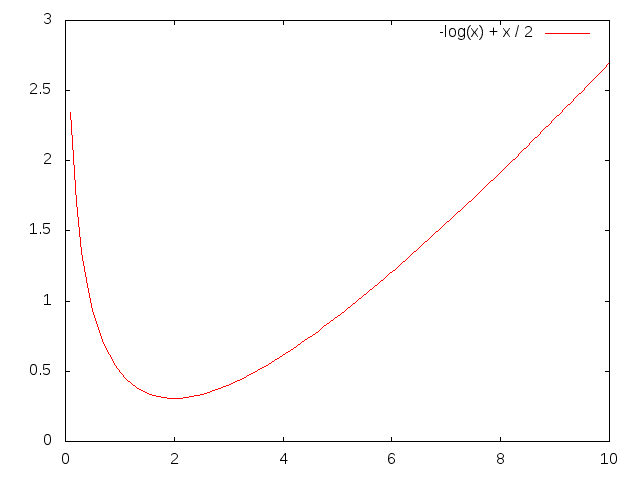
\includegraphics[width=.9\linewidth]{kullback-leibler.png}

\subsection{Sampling methods}
\label{sec-1-11}
\subsection{Continuous latent variables}
\label{sec-1-12}
\subsection{Sequential data}
\label{sec-1-13}
\subsection{Combining models}
\label{sec-1-14}
% Emacs 25.1.1 (Org mode 8.2.10)
\end{document}